\chapter[Input feature distributions]{Input feature distributions for the $e/\gamma$ identification BDT in the HGCAL L1T}\label{app:egid_features}
\vspace{-1.1cm}
\begin{figure}[htb!]
  \centering
  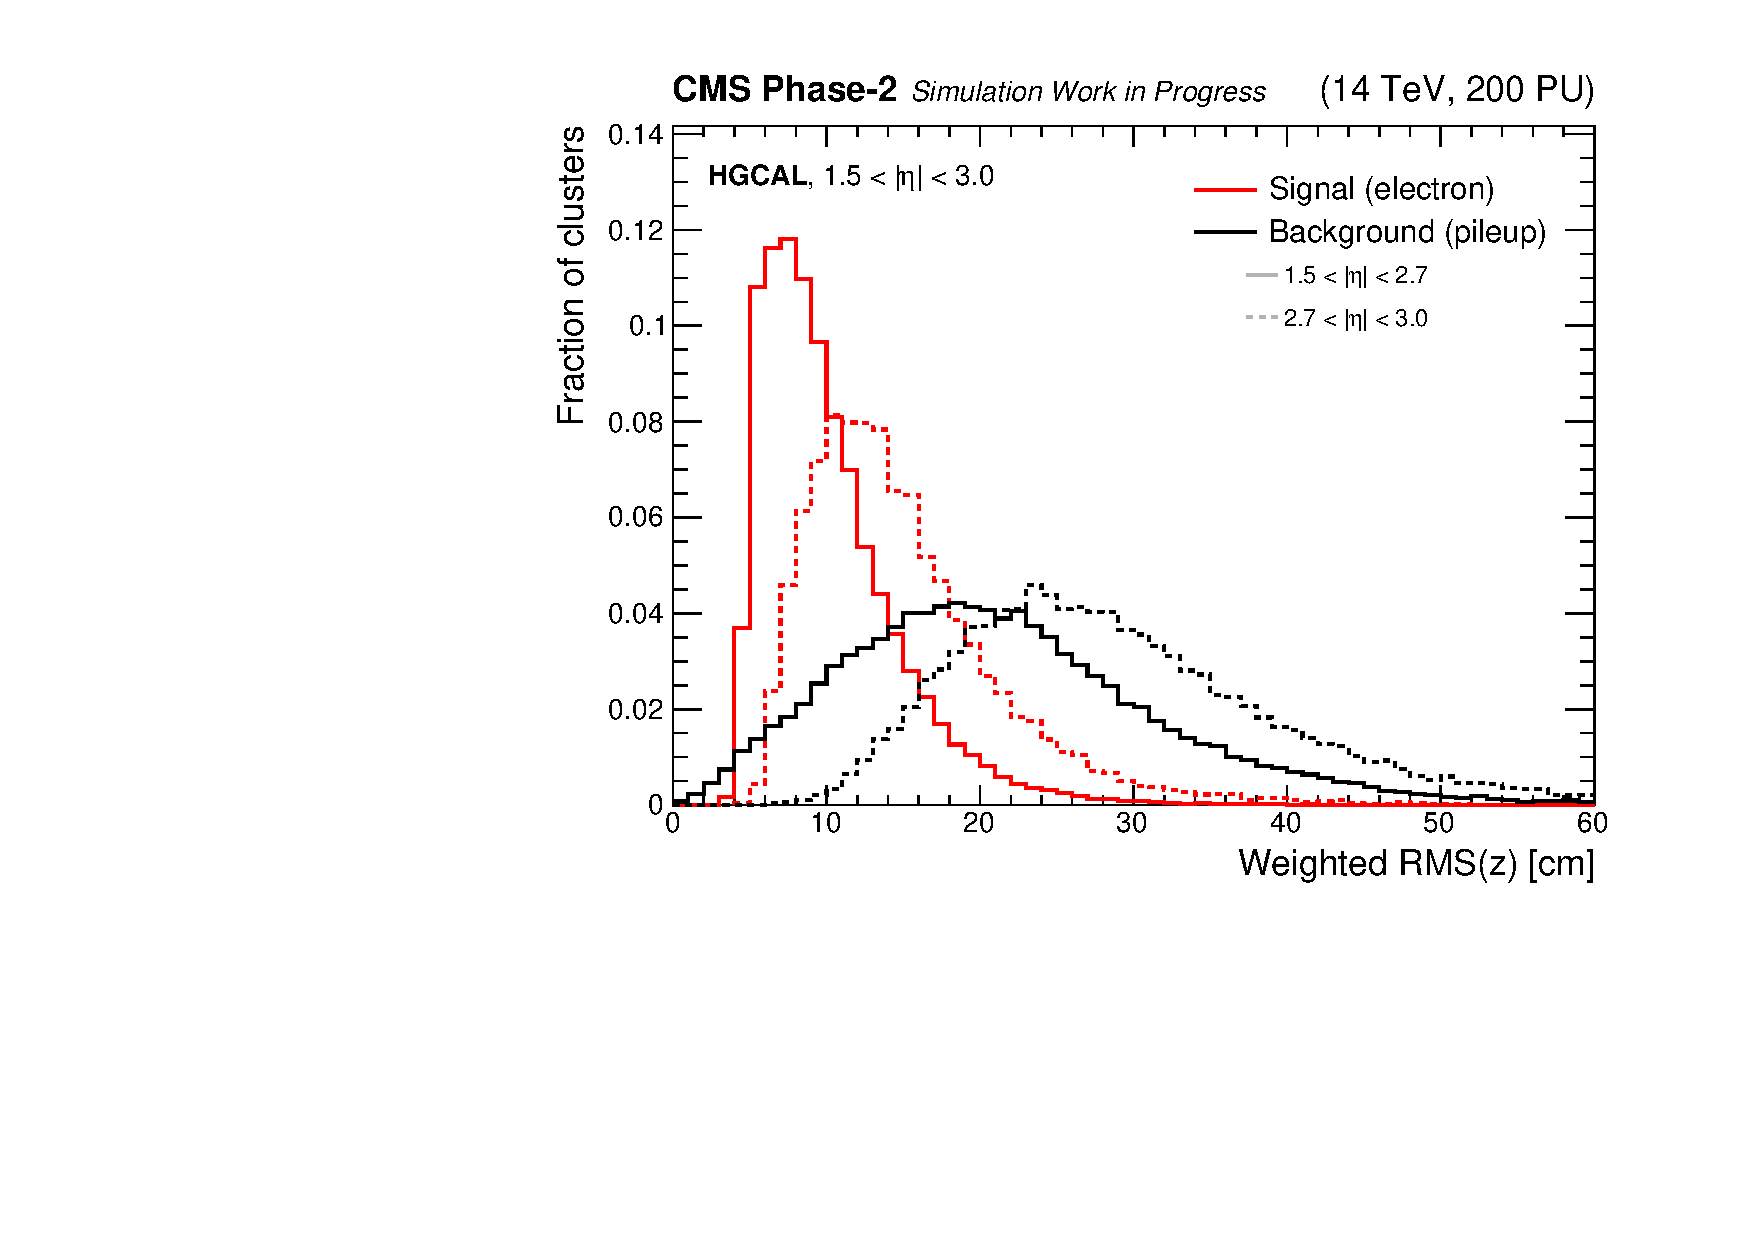
\includegraphics[width=.32\textwidth]{Figures/cms/egid/cl3d_szz.pdf}
  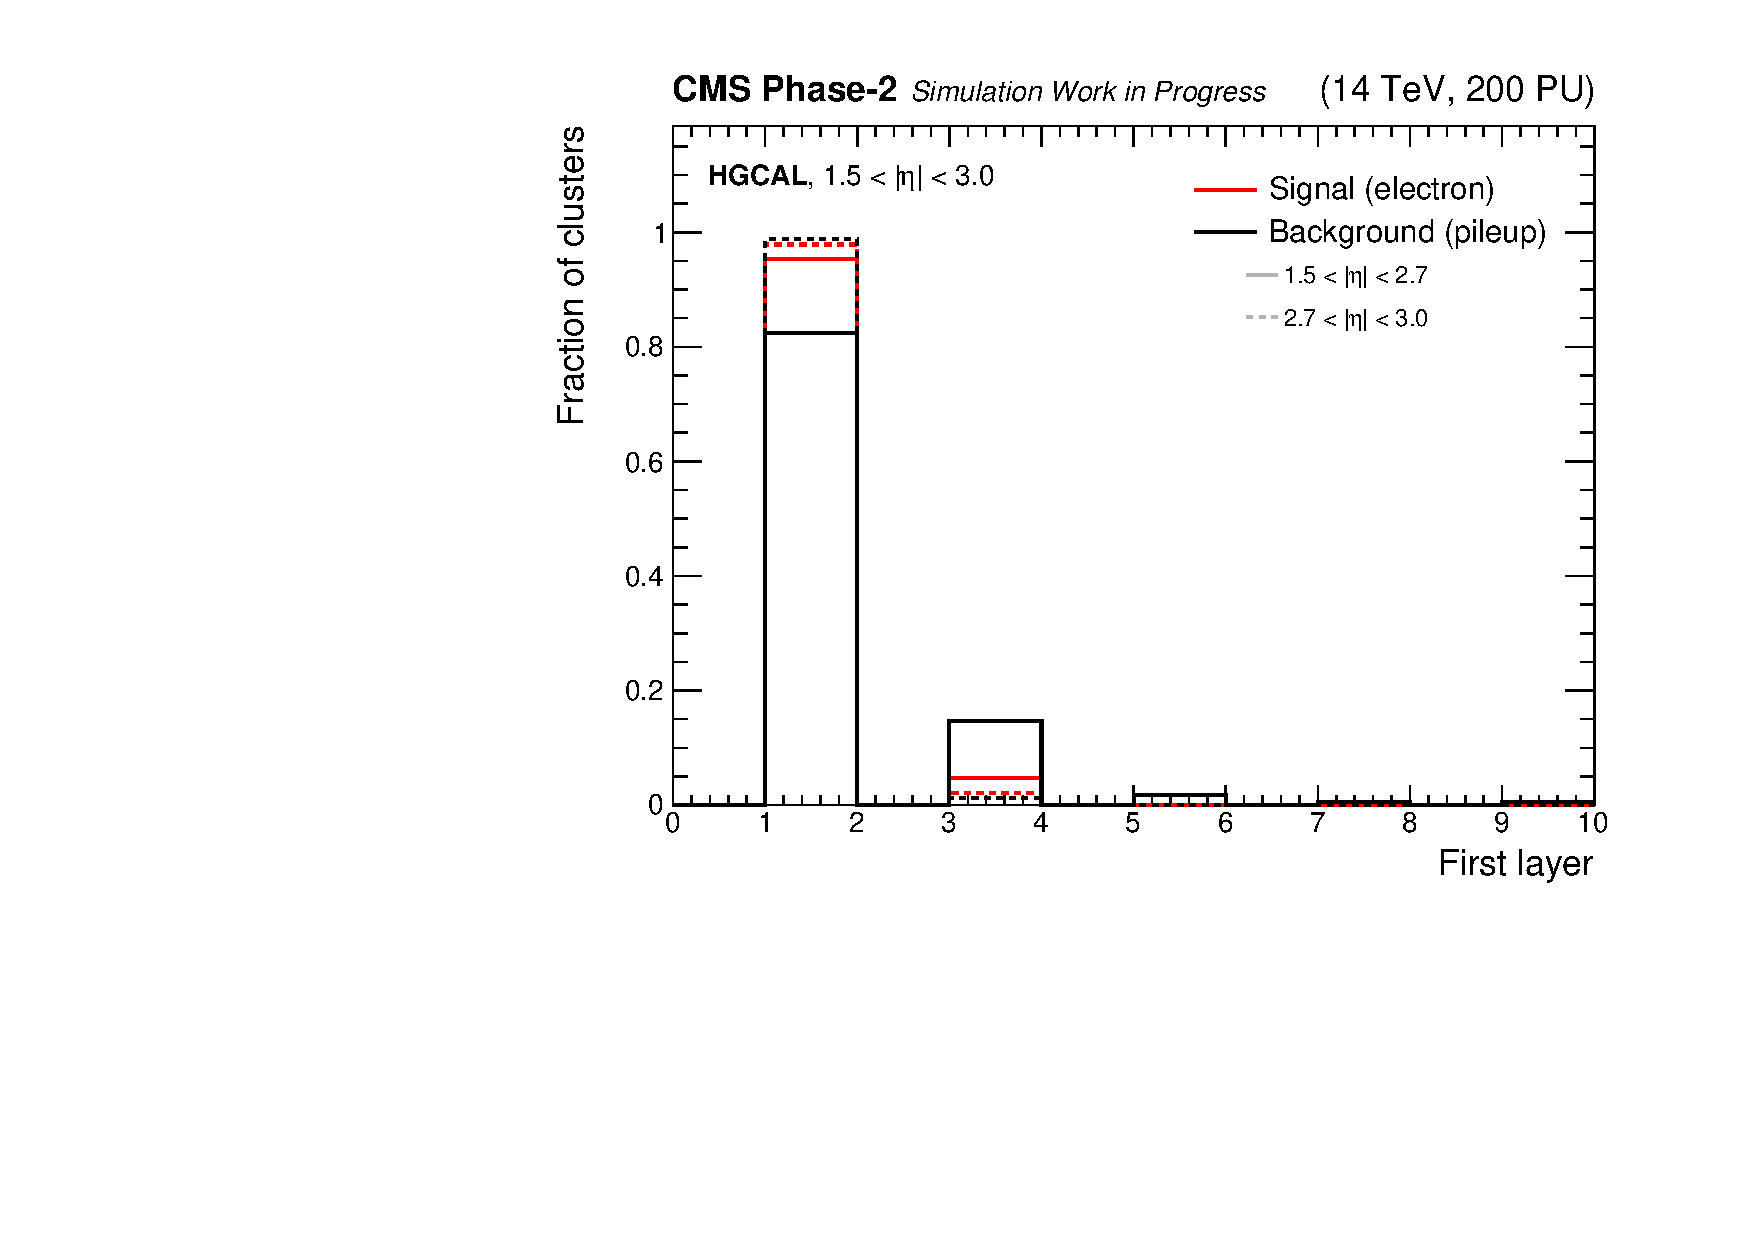
\includegraphics[width=.32\textwidth]{Figures/cms/egid/cl3d_firstlayer.pdf}
  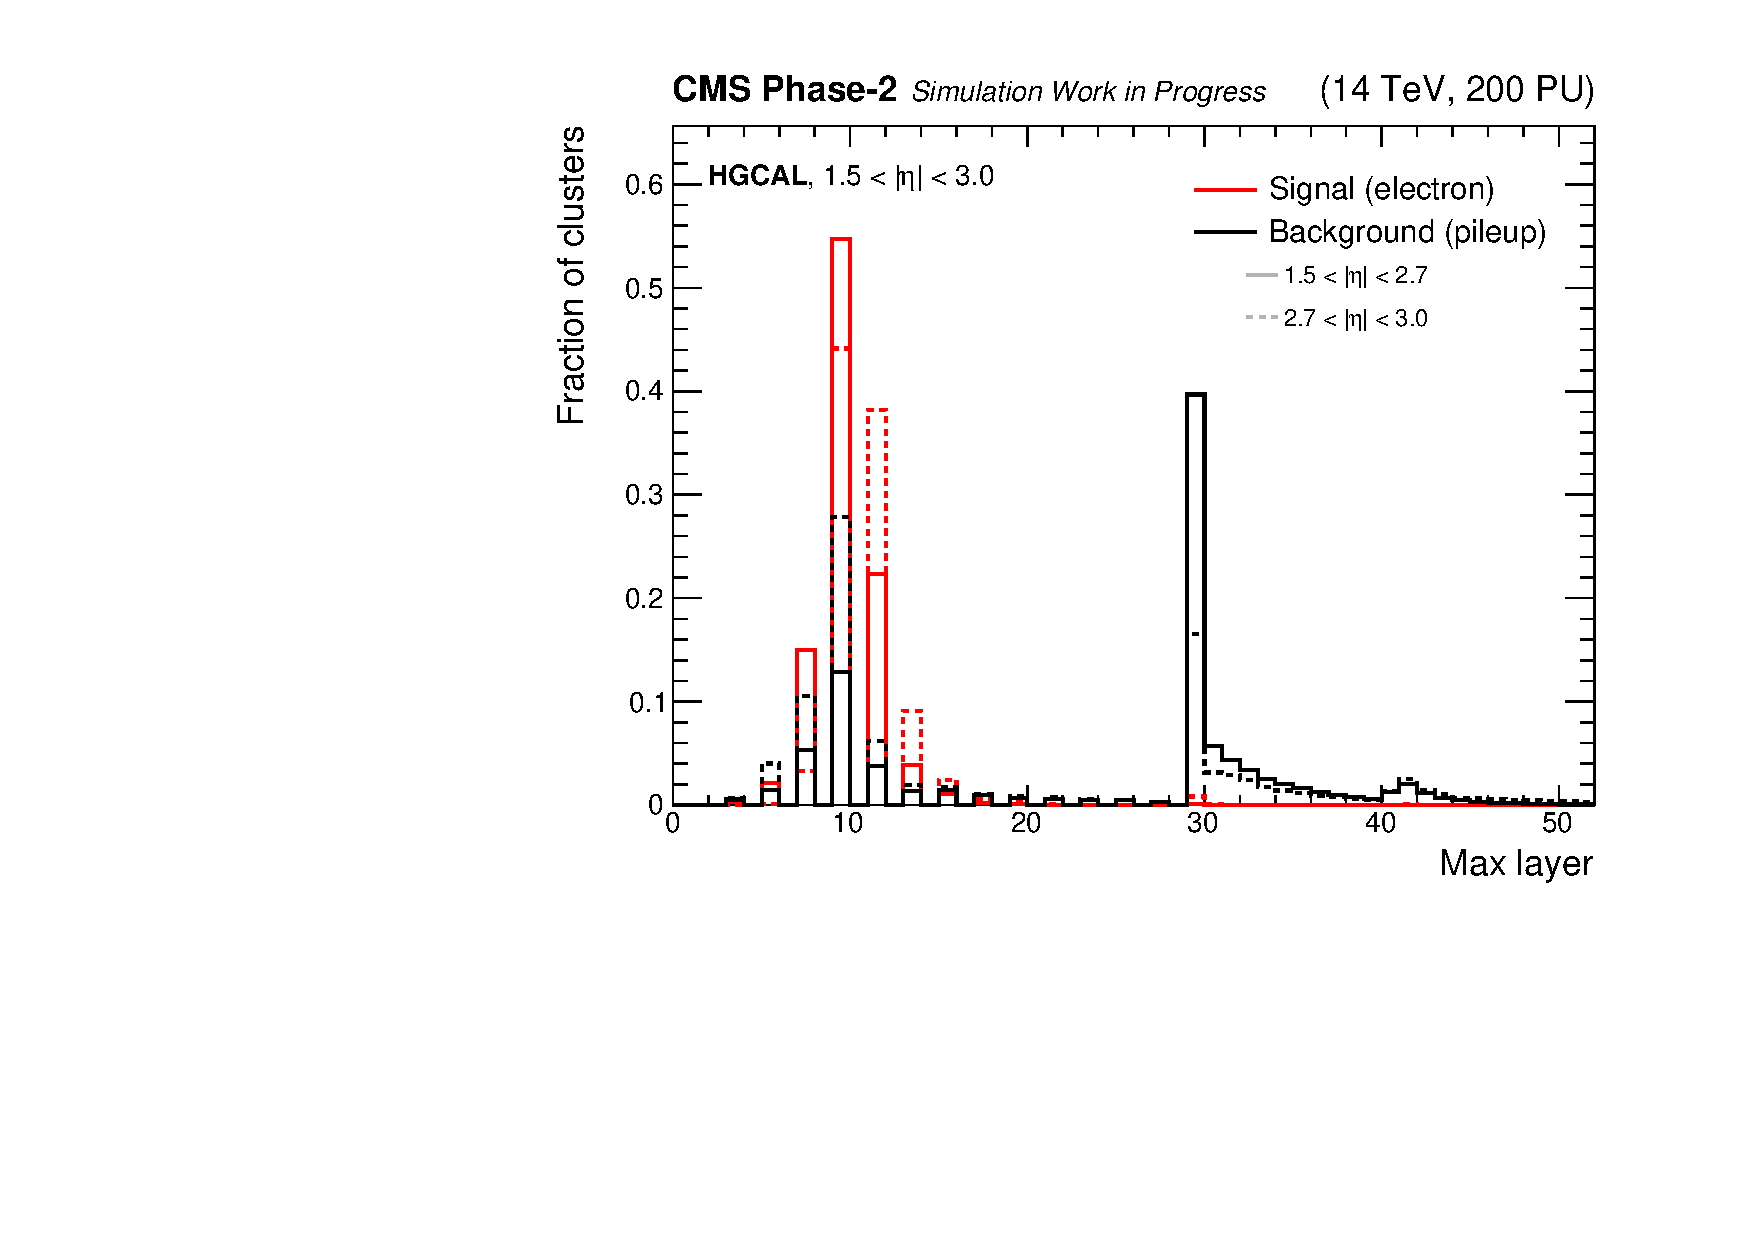
\includegraphics[width=.32\textwidth]{Figures/cms/egid/cl3d_maxlayer.pdf}
  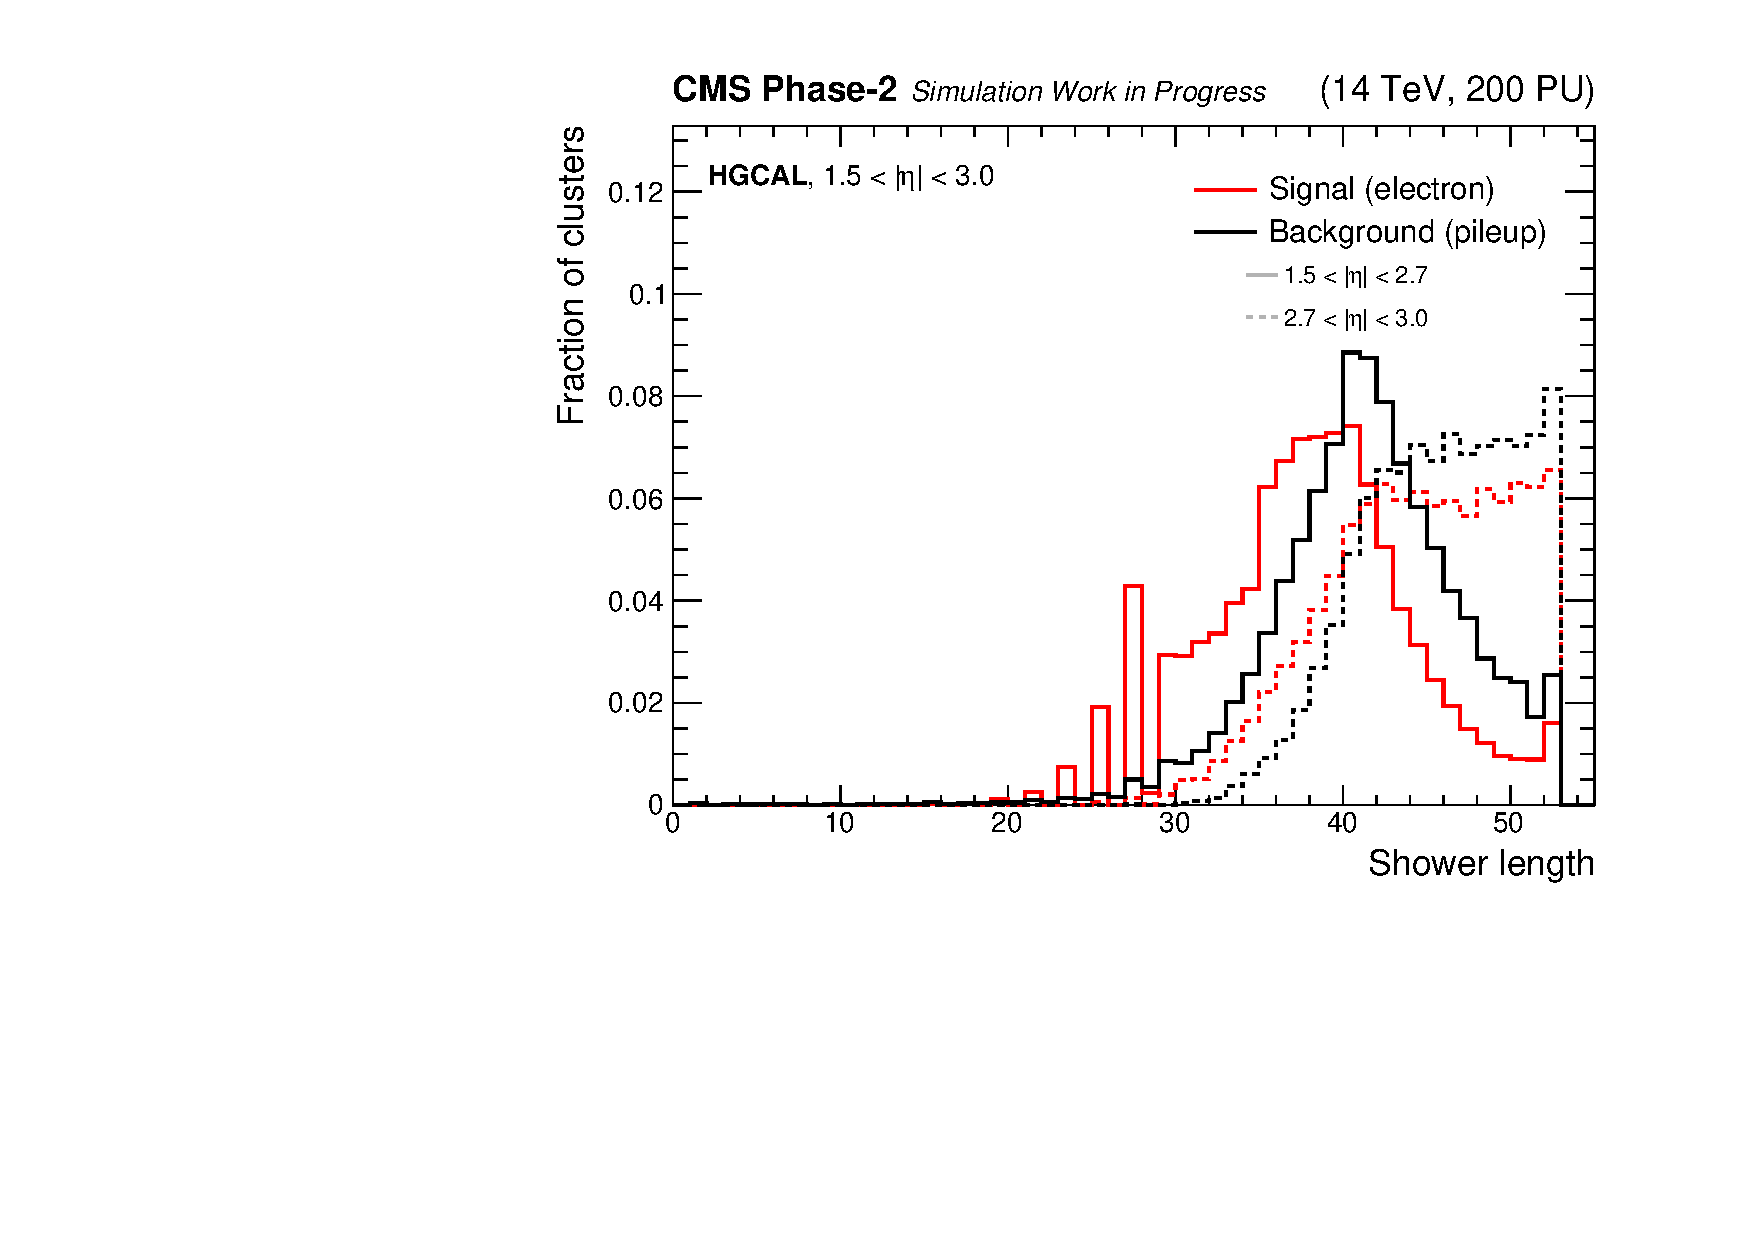
\includegraphics[width=.32\textwidth]{Figures/cms/egid/cl3d_showerlength.pdf}
  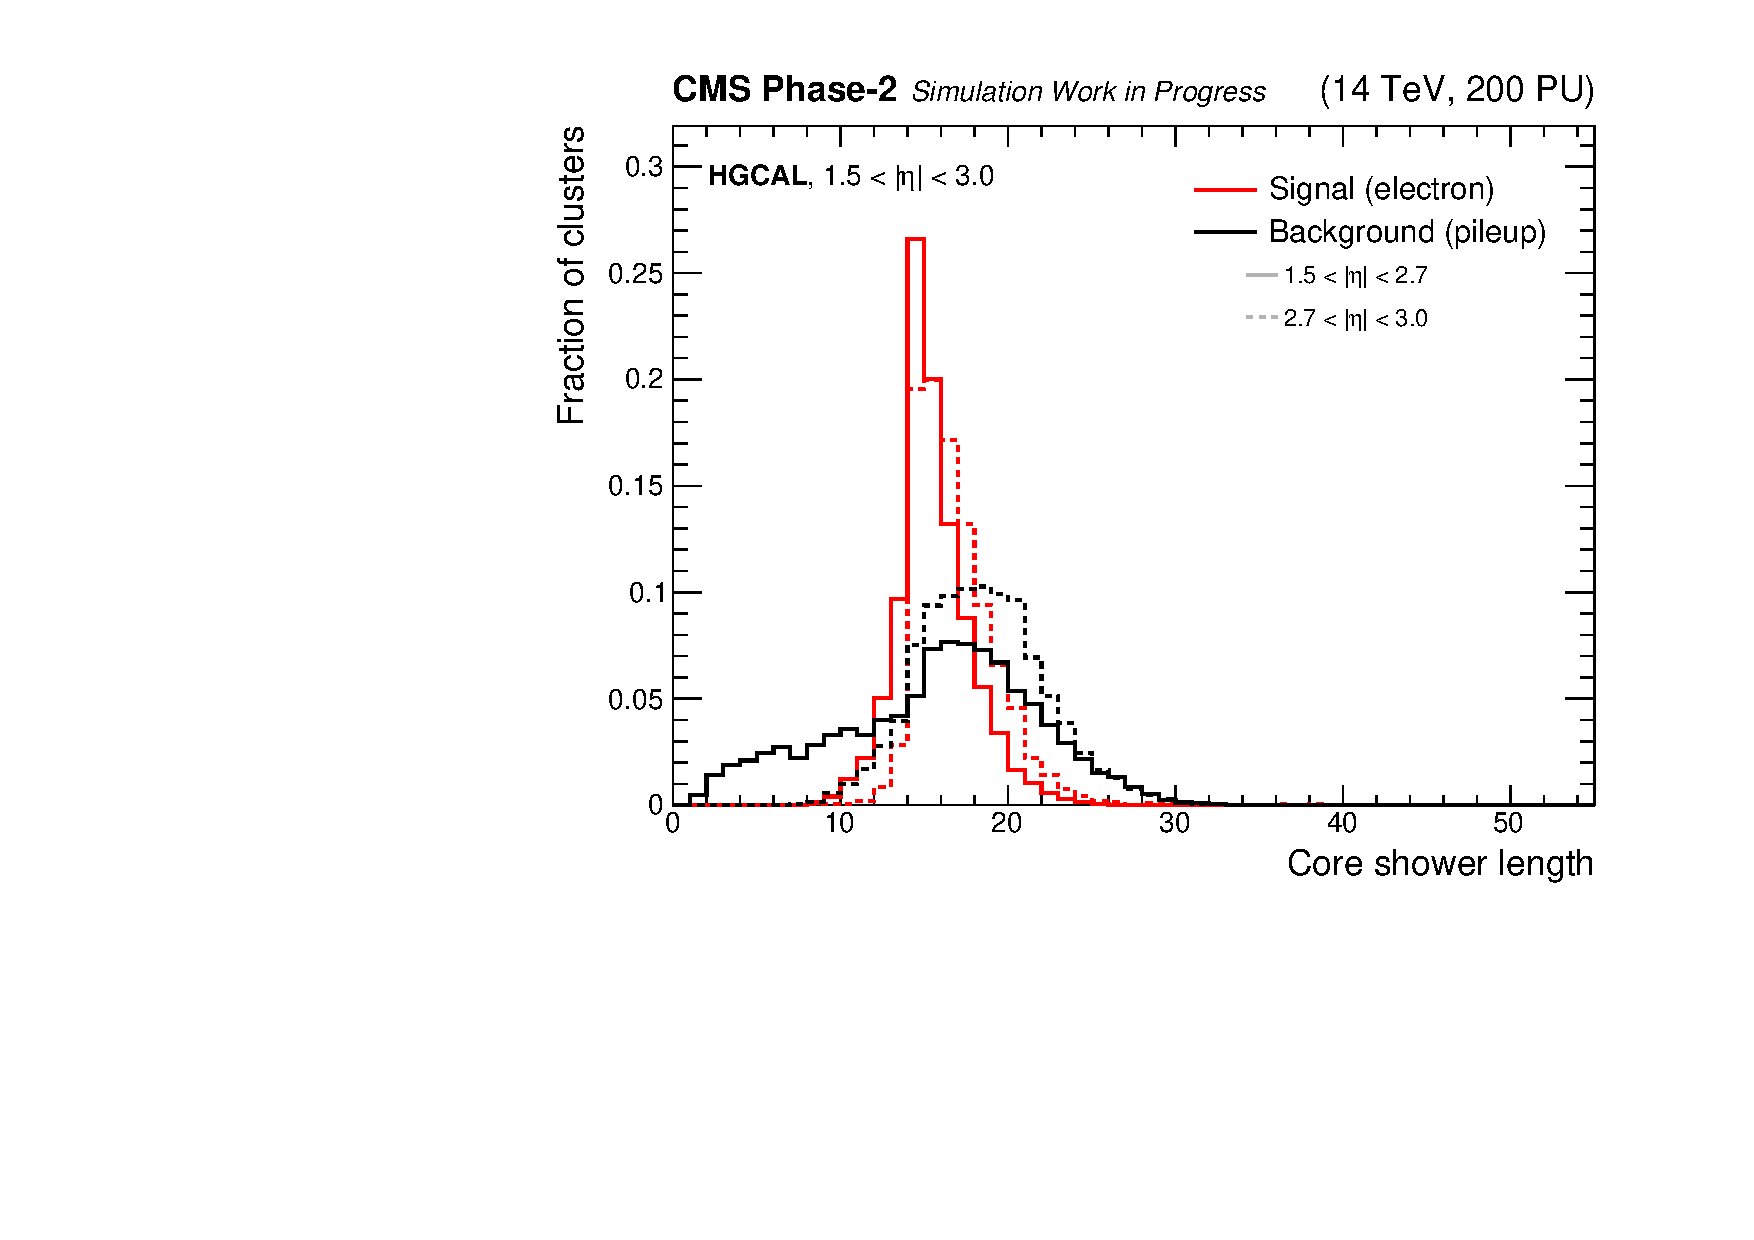
\includegraphics[width=.32\textwidth]{Figures/cms/egid/cl3d_coreshowerlength.pdf}
  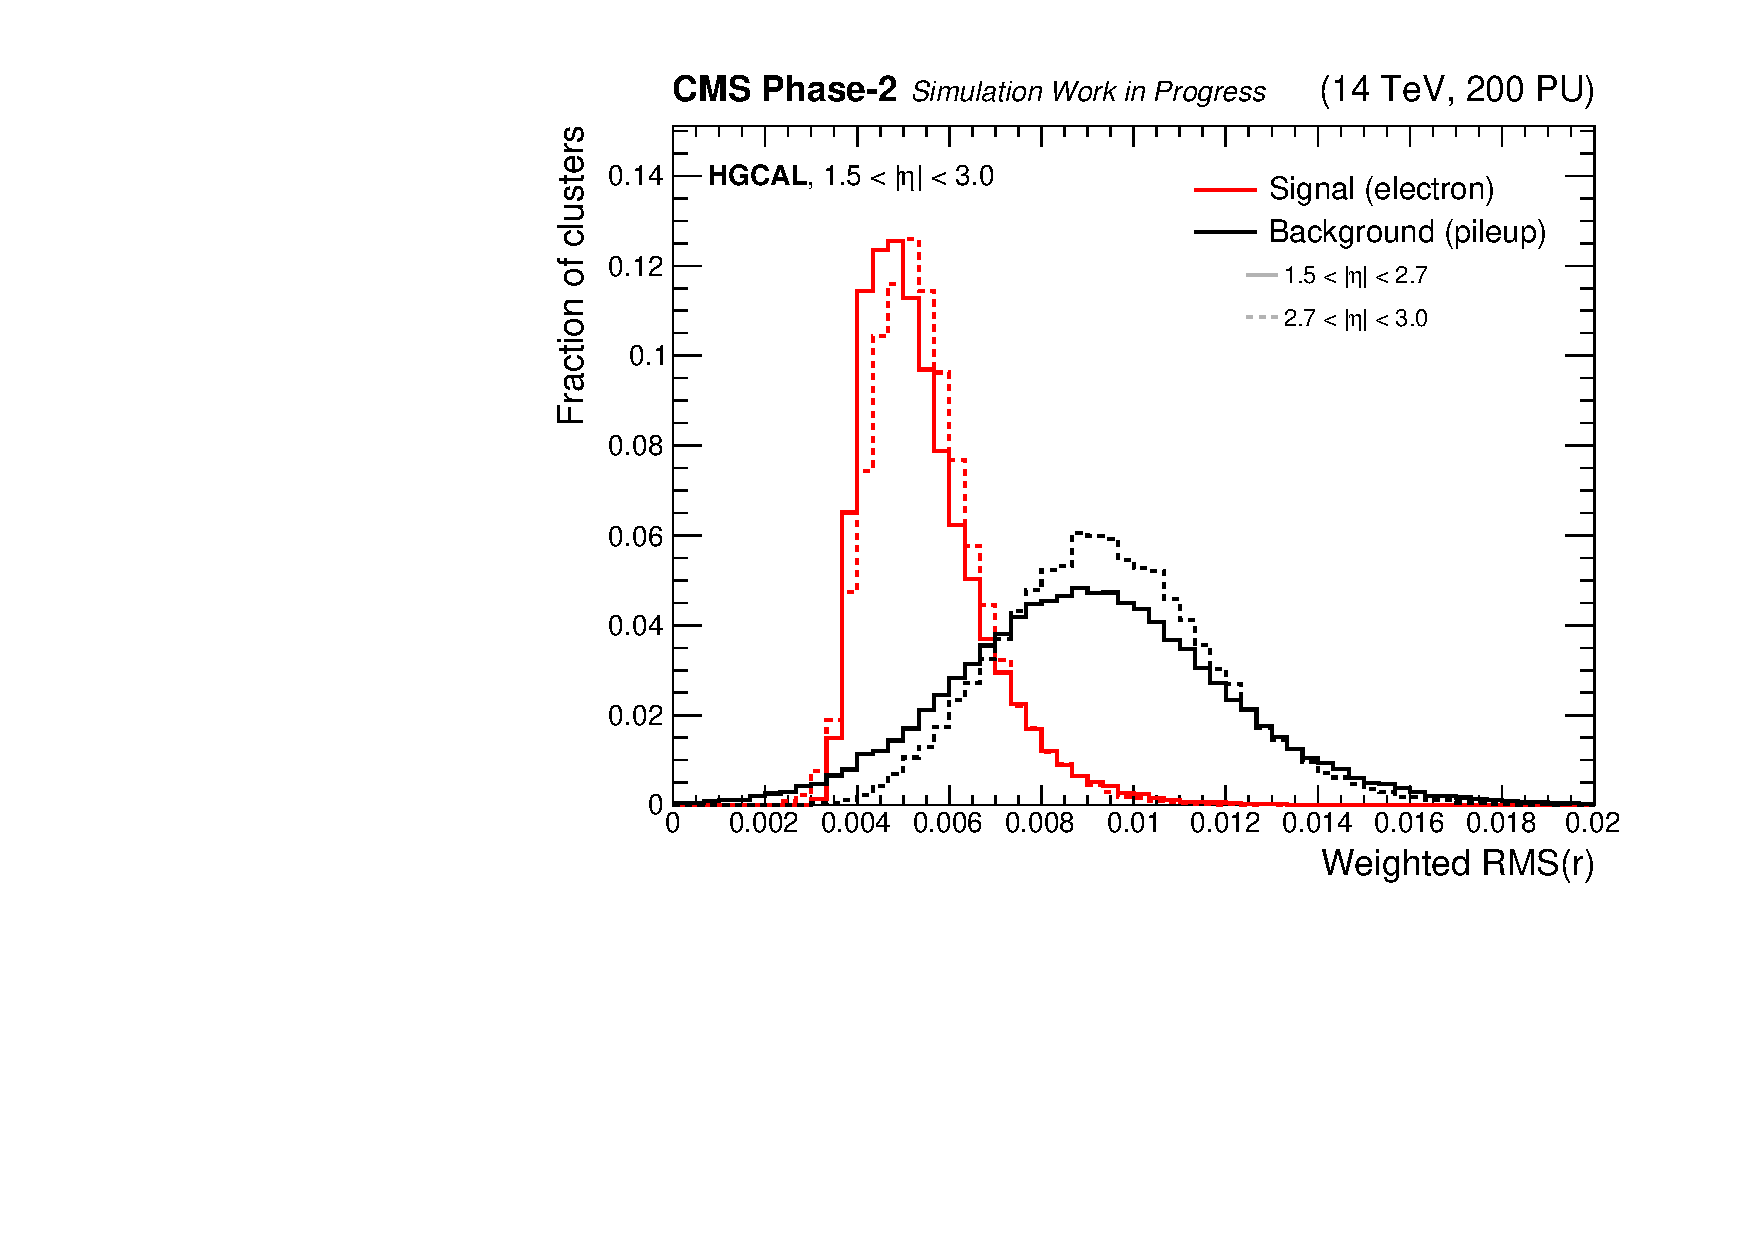
\includegraphics[width=.32\textwidth]{Figures/cms/egid/cl3d_srrtot.pdf}
  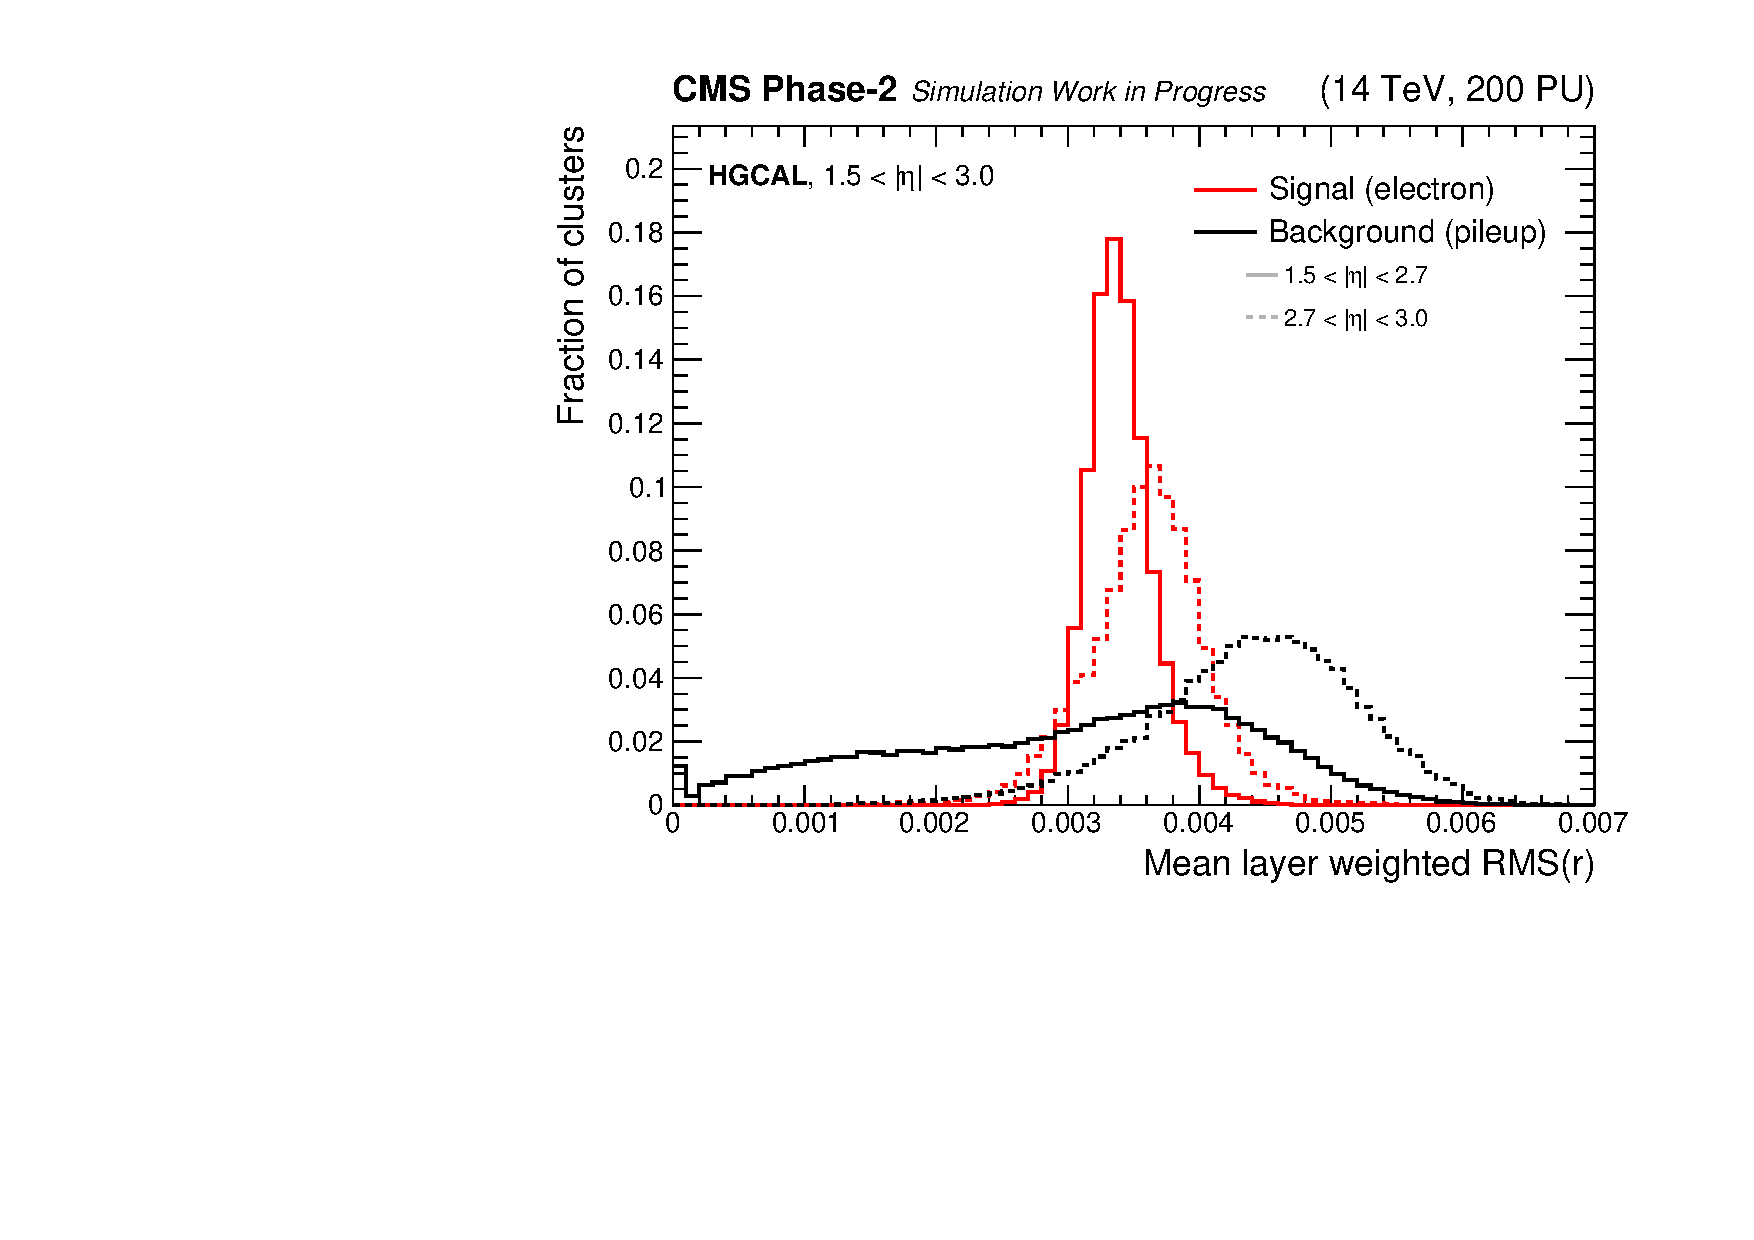
\includegraphics[width=.32\textwidth]{Figures/cms/egid/cl3d_srrmean.pdf}
  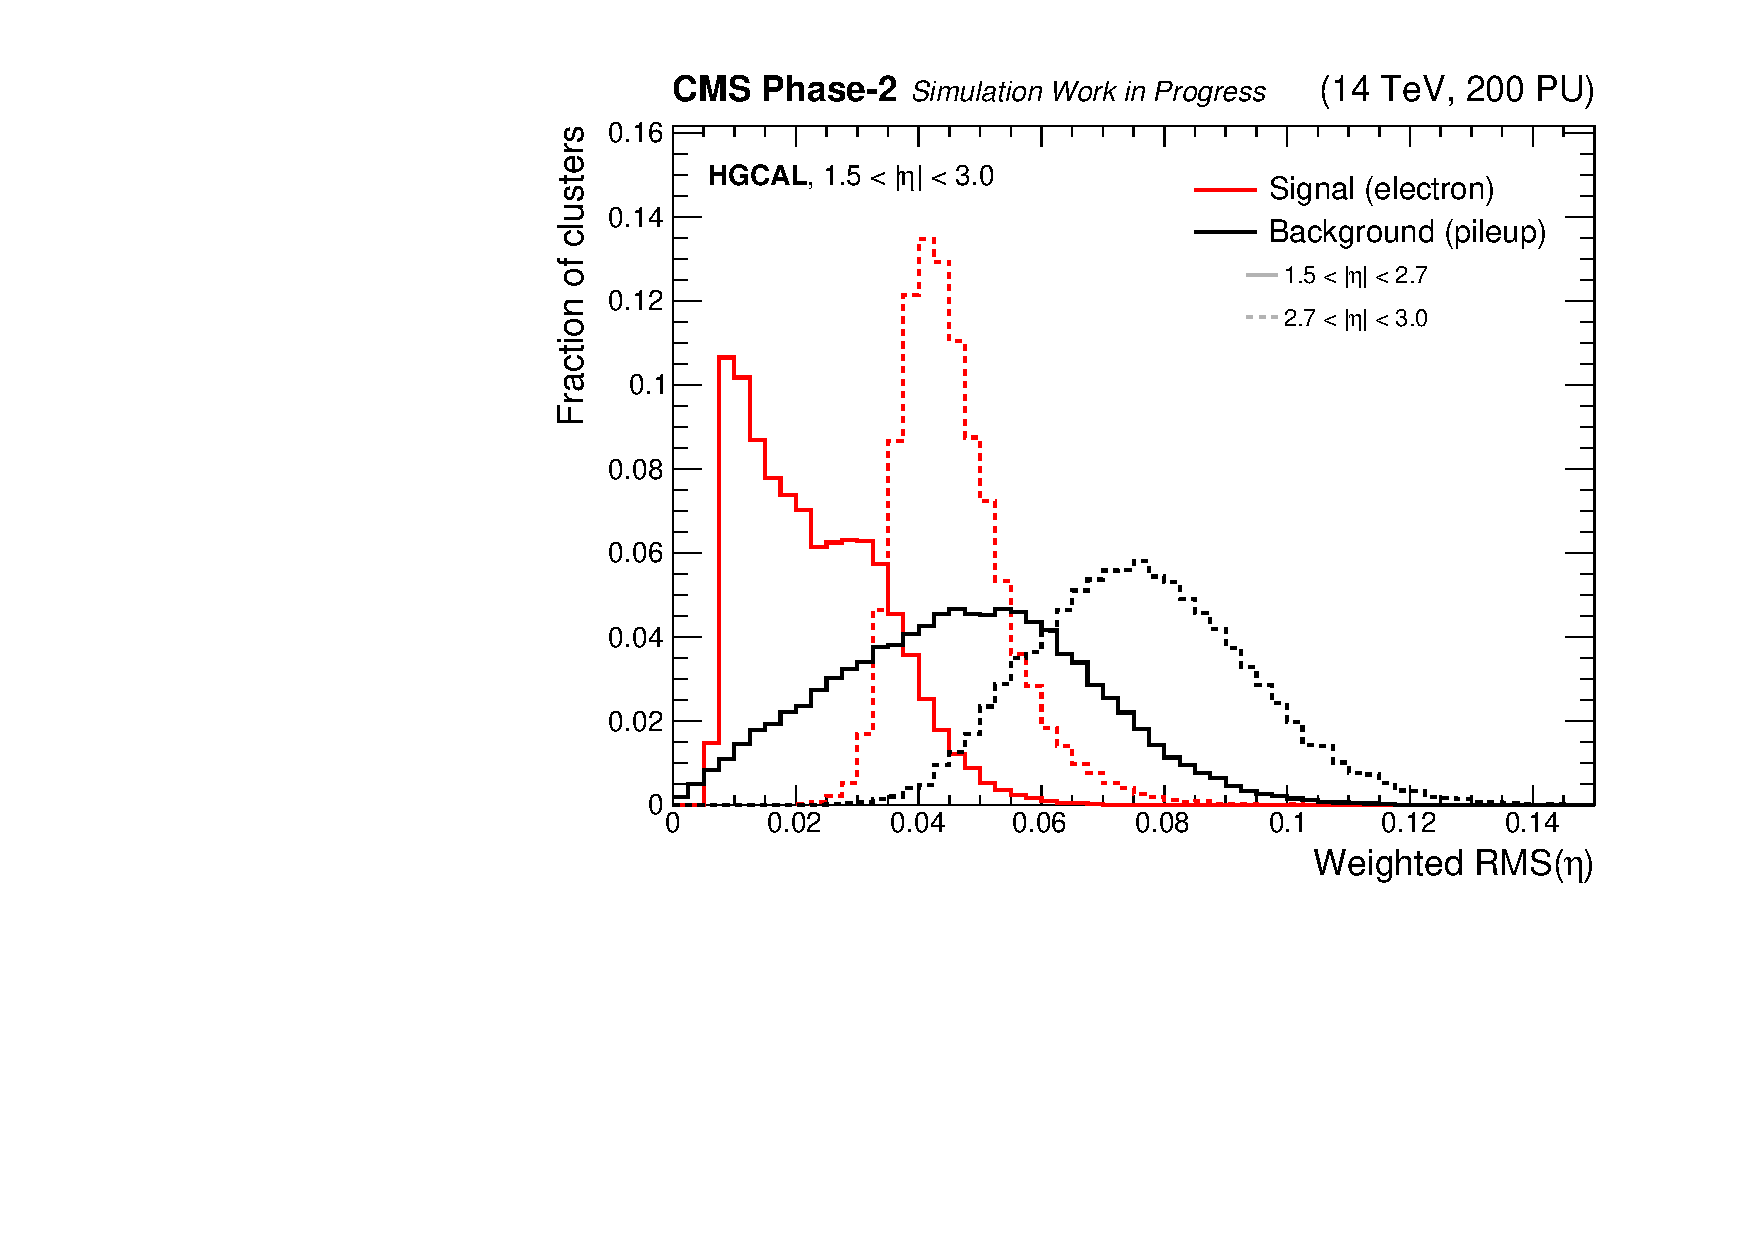
\includegraphics[width=.32\textwidth]{Figures/cms/egid/cl3d_seetot.pdf}
  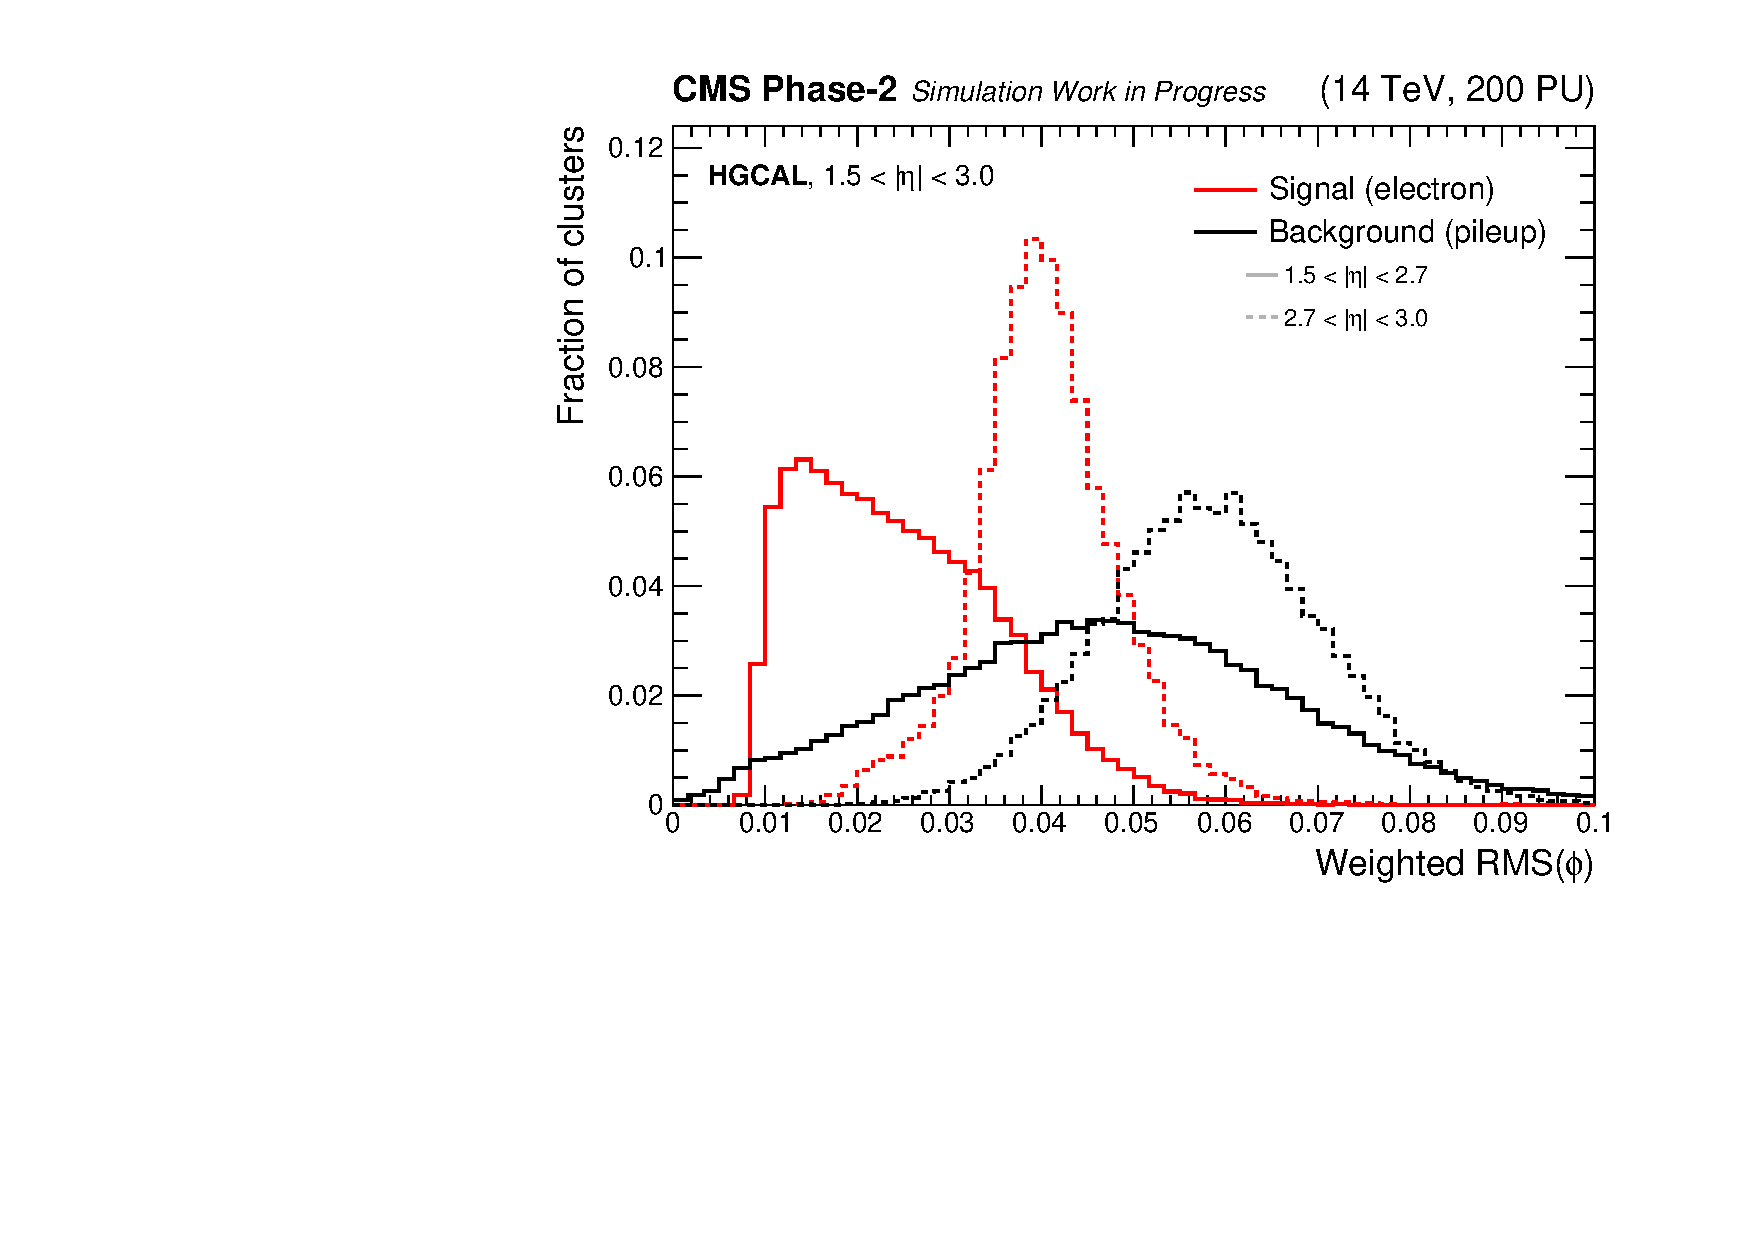
\includegraphics[width=.32\textwidth]{Figures/cms/egid/cl3d_spptot.pdf}
  \caption[$e/\gamma$ identification input feature distributions]
  {
    The distributions of the input features to the HGCAL L1T $e/\gamma$ identification BDT algorithm. The first five plots represent the five longitudinal shower shape variables, whilst the final four plots shows the four lateral shower shape variables. The signal clusters (generator-level matched electron) and background clusters (pileup) are shown in red and black respectively, and are separated into the two pseudorapidity regions in which the BDTs are trained.
  }
  \label{fig:egid_all_features}
\end{figure}